\chapter{Introduzione} \label{chap:introduzione}
	
	\mylettrine{C}{hiunque} abbia la seppur minima passione per la musica avrà sicuramente sentito parlare, al giorno d'oggi, del formato (o più in generale, della tecnologia) \textit{MP3}. Sicuramente i più sapranno che l'MP3 è un formato audio digitale che permette di memorizzare file audio, come canzoni, utilizzando molto meno spazio rispetto ai precedenti formati, pur mantenendo una buona qualità sonora: molti ricorderanno l'avvento dei primi lettori CD MP3, che permettevano di registrare e riprodurre centinaia di canzoni in un unico CD da 700 MB, al contrario delle massimo 20 canzoni che si potevano masterizzare in qualità CD (di queste differenze di formati e qualità audio parleremo ampiamente più avanti).\\
	La parola MP3 è spesso associata ai concetti di ``Internet'', ``frode'' o ``pirateria informatica'', dal momento che la sua venuta ha dato il via, o comunque incentivato, il download di enormi quantità di dati audio, spesso senza possedere alcuna licenza ed in modo certamente illegale.\\
	\\
	Ma a parte questi aspetti di conoscenza comune, pochi sanno veramente cos'è l'MP3 e come funzioni ed ancor meno sono quelli che si prendono la briga di spiegarlo. Con questo elaborato ci prefiggiamo quindi l'obiettivo di descrivere come e perché è nato l'MP3 e come esso funzioni, senza perdersi troppo nei dettagli tecnici ma fornendo comunque un'idea generale della tecnologia MP3.
	
	\section{Definizioni} \label{sec:definizioni}
		Senza dilungarci troppo nei dettagli, diamo alcune definizioni iniziali che faciliteranno la comprensione di questa relazione.
		
		\begin{defi} \label{defi:mp3}
			L'\emph{\textbf{MP3}} (ovvero \emph{\textbf{M}oving \textbf{P}icture} Expert Group-1/2 Layer \textbf{III}), detto anche \emph{MPEG-1/2 Layer III}, è un algoritmo di compressione audio di tipo \emph{lossy}, sviluppato dal gruppo \emph{MPEG}.
		\end{defi}
		
		Avendo introdotto, nella definizione precedente, il concetto di algoritmo \textit{lossy}, definiamo adesso cos'è un algoritmo di compressione \textit{lossy} e cos'è invece uno \textit{loosless}:
		
		\begin{defi} \label{defi:lossy}
			Un algoritmo di compressione \emph{\textbf{lossy}} è un metodo di codifica che comprime i dati scartandone alcuni. Tramite il processo di decodifica, quindi, non sarà possibile riottenere i dati originali.
		\end{defi}
		
		\begin{defi} \label{defi:loosless}
			Un algoritmo di compressione \emph{\textbf{loosless}} è un metodo di codifica che comprime i dati senza perderne alcuno. Tramite opportuna decodifica sarà quindi possibile ottenere nuovamente i dati originali.
		\end{defi}
		
		Già da queste definizioni possiamo dedurre che l'MP3 è un algoritmo di compressione audio che, comprimendo i dati, scarta alcune informazioni, al fine di rendere il file finale molto più leggero e maneggevole.
		
	\section{Cenni di compressione di dati} \label{sec:cenni_compressione_dati}
		
		Nel 1949 Claude E. Shannon provò, all'interno del suo articolo ``A Mathematical Theory of Communication'', che esiste un limite teorico alla compressione dei dati senza perdere informazione, ovvero comprimendo i dati con algoritmi loosless. Questo limite, detto \textit{tasso d'entropia}, dipende dalla probabilità di trovare determinate sequenze di bit: è possibile comprimere i dati con un tasso di compressione vicino al tasso d'entropia ed è matematicamente impossibile fare meglio.\\
		Per ottenere una maggior compressione dei dati è necessario utilizzare algoritmi lossy e quindi accettare di perdere parte dei dati.\\
		\\
		Di seguito esporremo tre codifiche di tipo loosless molto semplici, una delle quali, come vedremo, utilizzata anche all'interno dell'algoritmo di compressione e decompressione MP3.
		
		\subsection{Run-Length Encoding} \label{subsec:run-length_encoding}
		
			L'algoritmo di compressione loosless \textit{Run-Length Encoding} (o semplicemente \textit{RLE}) consiste nel codificare le varie sequenze di bit consecutivi aventi lo stesso valore come coppie, dove il primo elemento rappresenta il valore di quei bit e il secondo elemento indica il numero di bit che compongono la sequenza, ovvero la lunghezza della sequenza. In Figura \ref{fig:run-length_encoding} possiamo vedere un esempio della codifica RLE. Questa codifica è ideale per dati con lunghe sequenze di bit identici (quindi sconsigliato per dati casuali).
			
			\begin{figure}[h!]
				\centering
					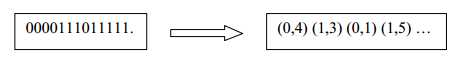
\includegraphics[scale=1]{run-length_encoding.png}
				\caption{Algoritmo di compressione Run-Length Encoding.}
				\label{fig:run-length_encoding}
			\end{figure}
			
		\subsection{Move-To-Front} \label{subsec:move-to-front}
			
			La codifica \textit{Move-To-Front} (o \textit{MTF}) si basa sul concetto di entropia ed infatti è ottimizzata quando la lettura di un carattere aumenta le probabilità di trovare lo stesso carattere subito dopo.\\
			L'algoritmo inizia codificando le lettere dell'alfabeto secondo l'ordine usuale (da 0 a 25). Quindi ogni carattere che viene incontrato viene spostato in cima alla lista. In generale, elementi in cima alla lista vengono codificati con meno bit, mentre quelli verso il fondo richiedono più bit.\\
			\\
			Se ad esempio prendiamo la parola ``BANANAAA'', la codifica MTF di questa parola sarà quella in Tabella \ref{tab:move-to-front}.
			
			\begin{table}[h!]
				\centering
				\begin{tabular}{|l|l|c|}
					\multicolumn{1}{c}{\textbf{Sequenza}} & \multicolumn{1}{c}{\textbf{Codifica}} & \multicolumn{1}{c}{\textbf{Lista}}\\
					\hline
					b & 1 & abcdefghijklmnopqrstuvwxyz\\
					\hline
					ba & 1, 1 & bacdefghijklmnopqrstuvwxyz\\
					\hline
					ban & 1, 1, 13 & abcdefghijklmnopqrstuvwxyz\\
					\hline
					bana & 1, 1, 13, 1 & nabcdefghijklmopqrstuvwxyz\\
					\hline
					banan & 1, 1, 13, 1, 1 & anbcdefghijklmopqrstuvwxyz\\
					\hline
					banana & 1, 1, 13, 1, 1, 1 & nabcdefghijklmopqrstuvwxyz\\
					\hline
					bananaa & 1, 1, 13, 1, 1, 1, 0 & anbcdefghijklmopqrstuvwxyz\\
					\hline
					bananaaa & 1, 1, 13, 1, 1, 1, 0, 0 & anbcdefghijklmopqrstuvwxyz\\
					\hline
				\end{tabular}
				\caption{Algoritmo di compressione Move-To-Front.}
				\label{tab:move-to-front}
			\end{table}
		
		\subsection{Codifica di Huffman} \label{subsec:codifica_huffman}
			
			Il concetto di entropia viene ampiamente applicato anche alla codifica di Huffman che, come vedremo più avanti, viene utilizzata all'interno dell'algoritmo di compressione MP3. L'idea che sta alla base della codifica di Huffman è quella di codificare con meno bit i caratteri più frequenti. La probabilità di incontrare determinati caratteri dev'essere determinata a priori (ad esempio analizzando i dati che si vogliono comprimere). Successivamente, in base alle probabilità calcolate, si assegnano codifiche più corte ai caratteri più frequenti e si memorizzano le associazioni carattere-codifica in una tabella, detta \textit{tabella di Huffman}, necessaria per la successiva decodifica dei dati. Come possiamo vedere in Figura \ref{fig:huffman}, la tabella di Huffman può essere rappresentata anche come un albero binario.
			
			\begin{figure}[h!]
				\centering
					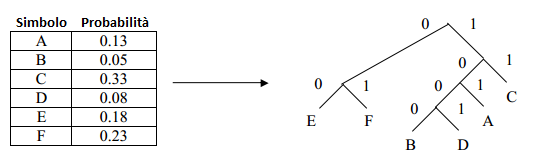
\includegraphics[scale=1]{huffman.png}
				\caption{Codifica di Huffman.}
				\label{fig:huffman}
			\end{figure}
		